\begin{tikzpicture}[scale=1.25]
\draw (0,4.5) -- (0,0.75) -- (1.8,.75);
%\node[anchor=south west] at (-0.9,-.2) {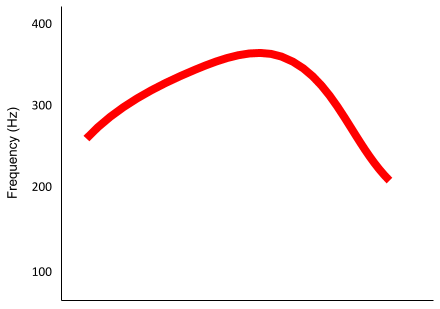
\includegraphics[scale=.4]{ranges-what-if1.png}};
\node[rotate=90] at (-0.75,2.2) {\relsize{-2}f0 (Hz)};
\begin{scope}[anchor=east, style={font=\relsize{-2}}]
	\node at (0,1) {100};
	\node at (0,2) {200};
	\node at (0,3) {300};
	\node at (0,4) {400};
\end{scope}
\foreach \y in {1,...,4}
{
	\draw (0,\y) -- (-.1,\y);
}

\draw[fill=CB1!40] (.3,1.35) rectangle (1.5,3.65);
\coordinate (pt1) at (0.925,3.6);
\coordinate (pt2) at (.825,3.57);
%
\coordinate (pt3) at (.885,3.48);
\coordinate (pt4) at (.933,3.23);
\coordinate (pt5) at (1.05,3);
\coordinate (pt6) at (0.85,2.9);
\coordinate (pt7) at (0.925,2.7);
%
\coordinate (pt8) at (.65,2.62);
\coordinate (pt9) at (0.75,2.58);
\coordinate (pt10) at (.85,2.6);
\coordinate (pt11) at (.95,2.6);
\coordinate (pt12) at (1.05,2.55);
\coordinate (pt13) at (1.15,2.65);
\foreach \x in {1,...,13}
{
\draw[fill] (pt\x) circle (.04);
}
%
\end{tikzpicture}